\section{Introduzione}
\subsection{ASGAL}
ASGAL (Alternative Splicing Graph ALigner) \cite{denti2018asgal} è un tool sviluppato dall'Algolab per l'identificazione di eventi di Alternative Splicing espressi in un campione di RNA-Seq a partire da un genoma di riferimento e dall'annotazione di un gene. ASGAL si compone di quattro step:

\begin{enumerate}
	\item \textbf{Costruzione dello splicing graph}: a partire dall'annotazione di un gene e dalla genomica di riferimento, ASGAL costruisce uno splicing graph, ovvero una struttura a grafo che rappresenta tutti i trascritti noti del gene in input. Viene inoltre prodotta una linearizzazione dello splicing graph, che sarà utilizzata in fase di allineamento.
	\item \textbf{Allineamento Splice-Aware}: utilizzando gli algoritmi in \cite{beretta2017mapping} e \cite{ohlebusch2010computing} ASGAL allinea le RNA-Seq reads con la linearizzazione dello splicing graph del gene in input. L'allineamento è Splice-Aware in quanto è necessario tenere traccia della posizione di esoni ed introni per un corretto allineamento.
	\item \textbf{Computazione degli allineamenti Spliced(opzionale)}: gli allineamenti ottenuti dall'Allineatore Splice-Aware vengono convertiti nel formato SAM, per permetterne l'elaborazione con strumenti standard.
	\item \textbf{Rilevazione degli eventi di Alternative Splicing}: gli allineamenti prodotti dall'Allineatore Splice-Aware sono analizzati per rilevare gli eventi di Alternative Splicing indotti dalle read del campione. Gli eventi rilevati sono visualizzati in un file csv, che include diverse informazioni su ciascun evento rilevato.
\end{enumerate}

ASGAL è stato sviluppato in C++ e Python: C++ viene utilizzato nella parte di allineamento per la sua efficienza, Python nella parte di rilevazione per la sua semplicità nell'utilizzo di strutture dati complesse. Il progetto è open source, ed è disponibile su GitHub con licenza GNU v3.0. Tutti i componenti sono utilizzabili singolarmente, ma viene fornito uno script principale che ne semplifica l'utilizzo.  

Al momento ASGAL non supporta le read paired-end, un nuovo formato di read prodotte da allineatori NGS (Next Generation Sequencing), che potrebbe portare ad un incremento di efficacia ed efficienza nella rilevazione di eventi di Alternative Splicing. 

%L'immagine nella pagina successiva riassume il funzionamento di ASGAL.

\begin{figure}[h!]
	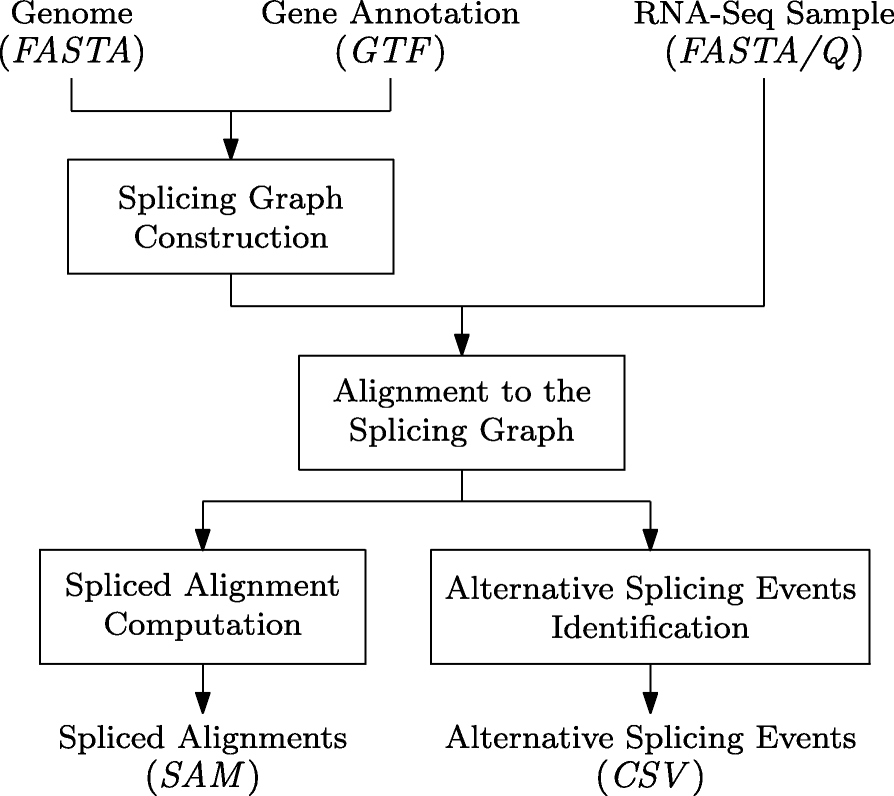
\includegraphics[width=\textwidth]{images/asgal.png}
  \caption{Il funzionamento di ASGAL illustrato}
  \label{fig:ASGAL}
\end{figure}
